\documentclass{beamer} 
\usetheme[hideothersubsections,width=2cm]{Berkeley}

\usepackage[utf8]{inputenc} 
\usepackage[francais]{babel} 
\usepackage{hyperref} 
\usepackage{textcomp} 
\usepackage{xcolor} 
\usepackage{graphicx} 
\usepackage{url} \urlstyle{sf}

\title{Programmation Neuro-Linguistique} 
\author{Geoffroy Carrier, J-Ch. Saad-Dupuy} \institute{Université Joseph Fourier, L3 MIAGE}

\date{23 février 2009}

\AtBeginSection[]
{
   \begin{frame}
       \frametitle{Plan}
       \tableofcontents[currentsection]
   \end{frame}
}

\begin{document}

\frame{
\titlepage}

\frame{ \frametitle{Plan} 
\tableofcontents }
\begin{frame}
	\frametitle{Kézako ?} Il existe énormément de définitions plus ou moins compatibles... \only<1>{
	\begin{block}
		{L'originale (Grinder \& Bandler)} 
		\begin{quote}
			A system of alternative therapy based on this which seeks to educate people in self-awareness and effective communication, and to change their patterns of mental and emotional behaviour. 
		\end{quote}
	\end{block}
	} \only<2>{
	\begin{block}
		{Simple et vague} 
		\begin{itemize}
			\item Étude de l'expérience subjective ; 
			\item Nouvelle approche de la communication et du changement ; 
			\item Nouvelle approche de la personnalité. 
		\end{itemize}
	\end{block}
	} \only<3>{
	\begin{block}
		{« Conceptuel »} 
		\begin{itemize}
			\item Étude de la structure de l’expérience subjective ; 
			\item Processus et modèle d'un processus ; 
			\item Modèle de l’expérience subjective ; et de la manière dont cette expérience influe sur notre comportement ; 
			\item Épistémologie de l'expérience. 
		\end{itemize}
	\end{block}
	} \only<4>{
	\begin{block}
		{Oxford English Dictionary (traduction libre)} 
		\begin{quote}
			Modèle de communication interpersonnelle principalement focalisé sur sur les motifs comportementaux à succès et les expériences subjectives sous-jacentes (particulièrement les motifs de pensée). 
		\end{quote}
	\end{block}
	} 
\end{frame}

\section{Origines}
\begin{frame}
	\frametitle{PNL} \only<1>{ Fondée dans les années 70 par John Grinder et Richard Bandler. } \only<2>{ Repose sur les travaux de 3 psychiatres : 
	\begin{itemize}
		\item Fritz Perls (Gestalt Therapy) ; 
		\item Virginia Satir (Thérapie familiale) ; 
		\item Milton Erickson (Hypnose Ericksonienne). 
	\end{itemize}
	} 
\end{frame}

\subsection{Gestalt Therapy}
\begin{frame}
	\frametitle{Gestalt Therapy} \only<1>{ 
	\begin{block}
		{Objectifs} 
		\begin{itemize}
			\item Augmenter la capacité d'adaptation à des êtres ou des environnements différents ; 
			\item Restaurer la liberté de choix de l'individu. 
		\end{itemize}
	\end{block}
	} \only<2>{ 
	\begin{block}
		{Résumé} Intègre cinq dimensions principales : 
		\begin{itemize}
			\item Physique ; 
			\item Affective : 
			\begin{itemize}
				\item Cognitive ; 
				\item Sociale ; 
				\item Spirituelle. 
			\end{itemize}
		\end{itemize}
	\end{block}
	} 
\end{frame}

\subsection{Thérapie familiale}
\begin{frame}
	\frametitle{La thérapie familiale} 
	\begin{block}
		{Résumé} 
		\begin{itemize}
			\item Les troubles d'un individu sont symptômes du dysfonctionnement dans lequel ce dernier évolue. 
			\item Thérapie intervenant sur tous les membres du groupe. 
		\end{itemize}
	\end{block}
\end{frame}

\subsection{Hypnose Ericksonienne}
\begin{frame}
	\frametitle{Hypnose Ericksonienne} \only<1>{
	\begin{block}
		{Résumé} 
		\begin{itemize}
			\item L'inconscient est profondement bon et puissant ; 
			\item Méthode de communication avec l'inconscient. 
		\end{itemize}
	\end{block}
	} \only<2>{
	\begin{block}
		{Champs d'application} 
		\begin{itemize}
			\item États depressifs ; 
			\item Phobies, angoisses ; 
			\item TOC ; 
			\item Dépendances ; 
			\item Travail sur le deuil ; 
			\item etc. 
		\end{itemize}
	\end{block}
	} \only<3>{
	\begin{block}
		{Objectif} Mobiliser le conscient et l'inconscient pour déclencher les changements utiles à la résolution d'une problématique. 
	\end{block}
	} 
\end{frame}

\section{Théorie}

\subsection{Bases}
\begin{frame}
	\frametitle{Méthode} 
	\begin{block}
		{Démarche itérative et « personnalisée »} 
		\begin{itemize}
			\item Diagnostic ; 
			\item Essai d'un modèle ; 
			\item Évaluation des résultats ; 
			\item Essai éventuel d'un autre modèle ; 
			\item Évaluation des résultats, etc. 
		\end{itemize}
		jusqu'à parvenir au résultat souhaité par le patient. 
	\end{block}
\end{frame}
\begin{frame}
	\frametitle{Experts en communication} 
	\begin{block}
		{Capacités} 
		\begin{itemize}
			\item Une acuité sensorielle développée ; 
			\item Une capacité à établir le rapport ; 
			\item Un respect réel du modèle du monde de l'autre ; 
			\item Un art de poser des questions précises ; 
			\item Beaucoup de flexibilité et d'adaptabilité ; 
			\item Une aptitude à établir et poursuivre des objectifs spécifiques. 
		\end{itemize}
	\end{block}
\end{frame}
\begin{frame}
	\frametitle{Fragments et aphorismes...} 
	\begin{itemize}
		\item On ne peut pas ne pas communiquer ; 
		\item Choisir d'influencer avec intégrité (écologique) ; 
		\item Être acteur ; 
		\item Utiliser le \emph{feedback} (retours d'informations) ; 
		\item Élargir sa vue ; 
		\item \emph{garde-fou de la PNL :} La carte n'est pas le territoire. 
	\end{itemize}
\end{frame}
\begin{frame}
	\frametitle{VAKOG} Canaux de communication issus des 5 sens : 
	\begin{itemize}
		\item Visuel ; 
		\item Auditif ; 
		\item Kinesthésique ; 
		\item Olfactif ; 
		\item Gustatif. 
	\end{itemize}
\end{frame}
\begin{frame}
	\frametitle{Mouvements occulaires} 
	\begin{center}
		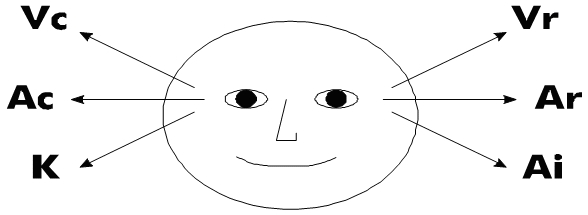
\includegraphics[width=8cm]{yeux.jpg} 
	\end{center}
	\begin{itemize}
		\item<+-> Vc : Visuel construit ; 
		\item<+-> Vr : Visuel remémoré ; 
		\item<+-> Ac : Auditif construit ; 
		\item<+-> Ar : Auditif remémoré ; 
		\item<+-> K : Kinesthésique ; 
		\item<+-> Ai : Auditif interne ou dialogue intérieur. 
	\end{itemize}
\end{frame}

\subsection{Techniques}
\begin{frame}
	\frametitle{Hors échange} 
	\begin{itemize}
		\item \emph{Swish Pattern} (fumeur) ; 
		\item Ancrage (madeleine) ; 
		\item Recadrage, négociation des parties, double dissociation, etc. 
	\end{itemize}
\end{frame}
\begin{frame}
	\frametitle{Synchronisation non-verbale} Miroir dans : 
	\begin{itemize}
		\item La posture ; 
		\item Les mouvements ; 
		\item Le ton ; 
		\item Le rythme de voix ; 
		\item La façon de respirer ! 
	\end{itemize}
\end{frame}
\begin{frame}
	\frametitle{Synchronisation verbale} 
	\begin{itemize}
		\item Reformulation ou écoute active ; 
		\item Synchronisation syntaxique (tournures de phrases) ; 
		\item Assortiment des prédicats (même canal sensoriel dominant). 
	\end{itemize}
\end{frame}
\begin{frame}
	\frametitle{Savoir ce que l'on veut} 
	\begin{block}
		{Viser un résultat...} 
		\begin{itemize}
			\item \emph{concret, spécifique, observable} ; 
			\item formulé en termes positifs (\emph{le cerveau ne peut se représenter la négation}) ; 
			\item conçu sous forme sensorielle (cible perceptible) ; 
			\item écologique (conciliant, calibré dans la relation). 
		\end{itemize}
	\end{block}
\end{frame}

\section{Limites et précautions}
\begin{frame}
	\frametitle{Dans l'entreprise} 
	\begin{itemize}
		\item<+-> En tant qu'outil, la PNL peut être se réveler enrichissante ; 
		\item<+-> En entreprise attention aux dérives, notamment au niveau : 
		\begin{itemize}
			\item du recrutement ; 
			\item des relations entre pairs ; 
			\item de l'évaluation. 
		\end{itemize}
	\end{itemize}
\end{frame}
\begin{frame}
	\frametitle{La MILS interpelle le législateur} Rapport MILS 2001 : \only<1>{ 
	\begin{quote}
		La programmation neurolinguistique, couramment dénommée PNL, forme un ensemble disparate de méthodes de communication (apprendre à reformuler un message, à décoder des signaux non verbaux, des mouvements oculaires, etc..), basé sur un ensemble tout aussi disparate de références théoriques. Les fondements scientifiques et les validations empiriques sont faibles~: les hypothèses relatives aux mouvements oculaires ont d'ailleurs été infirmées. 
	\end{quote}
	} \only<2>{ 
	\begin{quote}
		L'absence de principes déontologiques orientés vers l'aide et la santé, plutôt que vers l'exploitation et le profit, l'absence de connaissances en psychopathologie et en psychiatrie permettant d'aider ou d'orienter les personnes perturbées, l'absence de formation scientifique permettant de relativiser les connaissances et de ne pas prétendre à la vérité, caractérisent les pratiques qui font question. 
	\end{quote}
	} 
\end{frame}

\section{Références}
\begin{frame}
	\frametitle{Vous pouvez lire...} \only<1>{
	\begin{block}
		{Web (utiliser Google)} 
		\begin{itemize}
			\item Wikipedia anglophone, \emph{Neuro-linguistic programming} ; 
			\item Wikipedia francophone, \emph{Programmation neuro-linguistique} ; 
			\item \emph{Mieux communiquer avec la PNL pour atteindre ses objectifs} ; 
			\item \emph{La PNL : une pata-psychologie de plus} ; 
			\item \emph{La PNL ou l'art de manipuler ses semblables} ; 
			\item \emph{PNL} sur prevensectes. 
		\end{itemize}
	\end{block}
	} \only<2>{
	\begin{block}
		{Livres (utiliser Amazon)} 
		\begin{itemize}
			\item \emph{La PNL pour les Nuls} ; 
			\item \emph{Neuro-Linguistic Programming : volume 1 – The Study of the Structure of Subjective Experience} ; 
			\item \emph{Encyclopedia of Systemic Neuro-Linguistic Programming and NLP New Coding} ; 
			\item \emph{The structure of magic – tome 1}. 
		\end{itemize}
	\end{block}
	} 
\end{frame}

\end{document} 
